\section{Канцэпцыя праграмна-вызначаных сетак і асаблівасць іх рэалізацыі}

З'яўленне сеткі Інтэрнэт прывяло да стварэння лічбавага грамадства, у якім
амаль усе прылады злучаны паміж сабой і даступны з любога пункту свету.
Аднак нягледзячы на сваю распаўсюджанасць, сеткі IP маюць складаную структуру, і імі
давалі складана кіраваць. Такую сетку складана сканфігураваць для дасягнення выбранай
сеткавай палітыкі, а таксама рэканфігураваць у адпаведнасці са знойдзенымі недахопамі і
змяненнем нагрузкі і структуры. Да ўскладнення сітуацыі прыводзіць і тое, што сеткі,
якія ўжо існуюць, з'яўляюцца вертыкальна інтэграванымі: узровень кіравання сеткай і
ўзровень патока даных злучаны ў адзін.

Праграмна-вызначаная сетка (SDN) -- гэта канцэпт, які дае надзею на змяненне сітуацыі.
У такой сетцы адмаўляюцца ад вертыкальнай інтэграцыі, выносяць кантрольную логіку
за межы камутатараў і маршрутызатараў, а таксама ўносяць магчымасць праграмаваць сетку.
SDN спрашчае працэс стварэння і ўкаранення новых сеткавых абстракцый, пры гэтым
спрашчаючы кіраванне сеткай, і дапамагае эвалюцыі сеткі.

Каб апісаць высокаўзроўневыя палітыкі сеткі, аператары сеткі вымушаны канфіругаваць кожную
прыладу асобна, карыстаючыся нізкаўзроўневымі камандамі, якія часта адрозніваюцца ў
залежнасці ад вытворцы абсталявання. Акрамя таго, сеткавыя структуры павінны
вытрымліваць няспраўнасці і адаптавацца да змяненням узроўня нагрузкі.
Механізмаў аўмататычнай рэканфігурацыі практычна не існуе пры бягучым стане IP сетак.
Праз гэта ўскладняецца ўкараненне сеткавых палітык у такім пастаянна зменлівым асяроддзі.

Сучасныя сеткі таксама вертыкальна інтэграваныя, што толькі ўскладняе сітуацыю.
Узровень кіравання (які прымае рашэнне наконт апрацоўкі сеткавага трафіка) і
ўзровень даных (які накіроўвае трафік адпаведна рашэнням узроўня кіравання) звязаны
ўнутры сеткавай прылады, што змяншае гібкасць і перашкаджае інавацыям і эвалюціі
сеткавай інфраструктуры.

Праграмна-вызначаная сетка з'яўляецца канцэпцыяй, якая яшчэ развіваецца, якая дае надзею
на змяненне абмежаванняў сучасных сеткавых структур.
Па-першае, яна разбівае вертыкальную інтэграцыю, гэта значыць адасабляе логіку кіравання
(узровень кіравання) ад маршрутызатараў і камутатараў, якія накіроўваюць трафік (узровень даных).
Па-другое, з падзелам гэтых узроўняў, камутатары становяцца простымі прыладамі для маршрутызацыі,
а кіраванне сканцэнтравана ў лагічным цэнтралізаваным кантролеры (сеткавая аперацыйная сістэма),
што спрашчае ўвядзенне сеткавых палітык, рэканфігурацыю сеткі і яе эвалюцыю.
Спрошчаны від такой архітэктуры паказаны на малюнку \ref{img: Simple Infrastructure}.

\clearpage

\begin{figure}[ht!]
    \centering
    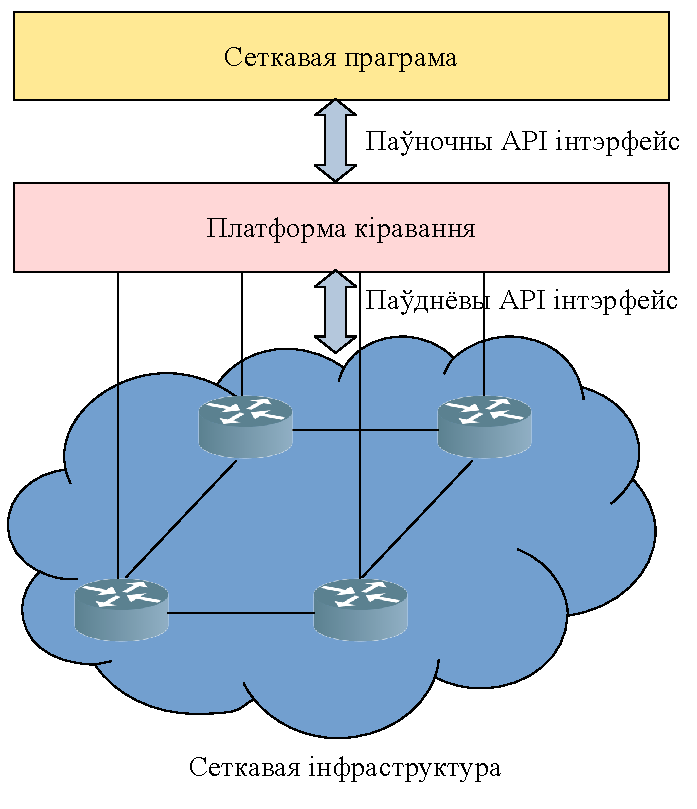
\includegraphics[width=0.5\textwidth]{simple_infrastructure.pdf}
    \vspace{-\baselineskip}
    \caption{Спрошчаны выгляд архітэктуры SDN}
    \label{img: Simple Infrastructure}
\end{figure}

Трэба адзначыць, што лагічна цэнтралізаваная мадэль не азначае фізічна цэнтралізаваную сістэму.
Насамрэч, для забеспячэння адпаведных узроўняў хуткадзейнасці, маштабавання і надзейнасці,
ад таіх рашэнняў трэба адмовіцца. Замест гэтага, SDN сеткі апіраюцца на фізічна размеркаваныя
ўзроўні кіравання.

Падзел двух гэтых узроўняў з'яўляецца ключом да дасягнення жаданай гібкасці сеткі,
адначасова разбіваючы праблему кіравання сеткай на лёгкія падзадачы і спрашчаючы ўвядзенне новых абстракцый.

\subsection{Азначэнне праграмна-вызначаных сетак}

Тэрмін праграмна-вызначанай сеткі (SDN) першапачаткова выкарыстоўваўся для апісання
працы вакол OpenFlow у Стэндфардскім Універсітэце.
Па першапачатковым азначэнні, SDN вызначае
cеткавую архітэктуру, у якой стан руху трафіка на ўзроўні даных
знаходзіцца пад кантролем  незалежнага ўзроўня кіравання.
Мы дадзім азначэнне SDN як сеткавай архітэктуры з
чатырма асаблівасцямі:
\begin{enumerate}
    \item узроўні кіравання і даных падзеляныя. Функцыі кіравання выдалены з сеткавых прылад, якія ста
новятся простымі элементамі маршрутызацыі;
    \item выкарыстоўваецца маршрутызацыя з улікам уласцівасці патока, а не канчатковага вузла прызначэння. Паток, у шырокім сэнсе -- гэта набор пэўных значэнняў у загалоўку пакета,
які служыць для выбару асобных пакетаў з агульнага трафіку і стварэння для іх адпаведных інструкцый.
У кантэксце SDN/Openflow, паток - гэта паслядоўнасць пакетаў паміж крыніцай і пунктам прызначэння.
Усе пакеты аднаго патоку атрымліваюць аднолькавы сeрвіс, адпаведведныя сеткавым палітыкам на прыладах маршрутызацыі.
    \item логіка кіравання перанесена ў асобны знешні аб'ект, так званы кантролер SDN або сеткавая аперацыйная сістэма (Network Operating System). NOS уяўляе сабой праграмную платформу, якая запускаецца на серверах і дае асноўныя рэсурсы для палягчэння праграмавання сеткавых прылад, грунтуючыся на лагічна
цэнтралізаваным, абстрактным плане сеткі.
    \item сетка можа быць запраграмавана пры дапамозе праграм, якія запушчаны на
    сеткавай аперацыйнай сістэме, якія ўзаемадзейнічаюць з прыладамі ўзроўня даных.
    Гэта з'яўляецца асноўнай характарыстыкай SDN, якая лічыцца галоўнай перавагай.
\end{enumerate}

\subsection{Агляд архітэктуры SDN}

Архітэктура SDN можа быць прадстаўлена як рад узроўняў (малюнак \ref{img: Layers}).
У кожнага ўзроўня ёсць свае спецыфічныя функцыі.
\begin{figure}[ht!]
    \centering
    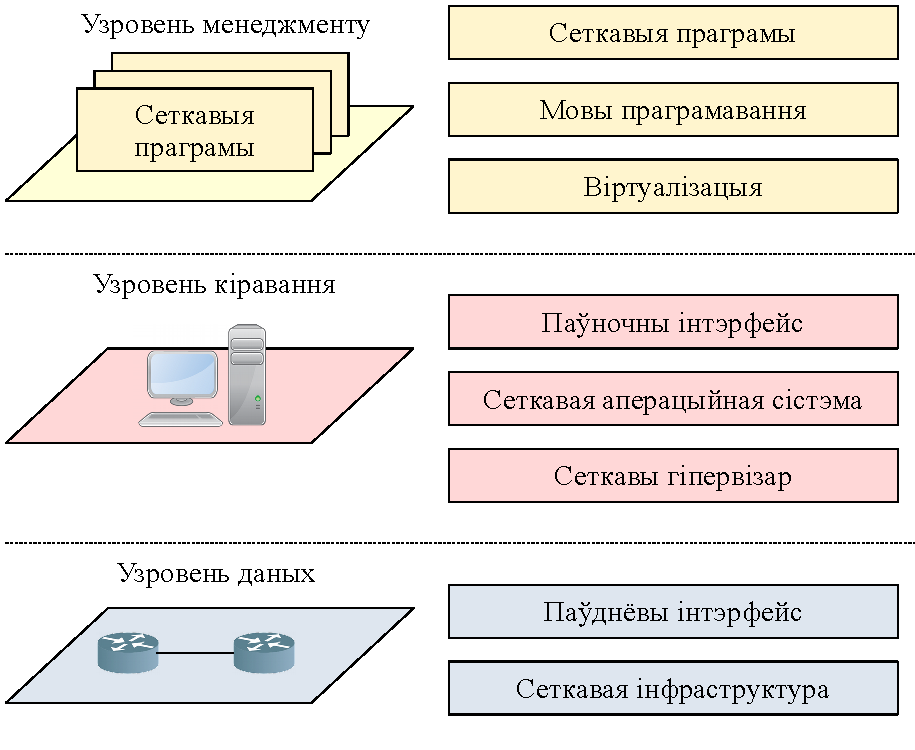
\includegraphics[width=0.7\textwidth]{layers.pdf}
    \vspace{-\baselineskip}
    \caption{Структура SDN сетак у выглядзе ўзроўняў}
    \label{img: Layers}
\end{figure}

Узровень даных (Data Plane): сеткавыя прылады злучаны па бесправадному альбо
правадному каналу сувязі. Сеткавая інфраструктура змяшчае ў сябе ўзаемазвязаныя
сеткавыя прылады, якія прадстаўляюць сабой узровень даных.

Узровень кіравання (Control Plane): сеткавыя прылады праграмуюцца элементамі
ўзроўня кіравання пры дапамозе паўночнага інтэрфейса. Узровень кіравання
можа лічыцца "мазгамі сеткі", Уся логіка кіравання знаходзіцца ў праграмах і кантролерах,
якія фарміруюць узровень кіравання.

Узровень менеджменту (Management Plane): гэты ўзровень прадастаўляе сабой
набор праграм, якія выконваюць функцыі паўночнага інтэрфейса для забеспячэння
кіравання сеткай. Такія праграмы ўключаюць у сябе маршрутызацыію, фаерволы,
размеркавальнікі нагрузкі, маніторынг і гэтак далей.
Праграмы менеджменту вызначаюць палітыкі, якія ў канцы канцоў інтэрпрэтыруюцца
як інструкцыі для паўднёвага інтэрфейса.

Разгледзім складкіні ўзроўня кіравання.

\subsubsection{Сеткавыя праграмы кіравання аперацыйнымі сістэмамі (Hypervisor).}
У сучасных кампьютарах тэхналогія віртуалізацыі не новая.
Хуткі рост прадукцыйнасці ў апошняе дзесяцігоддзе зрабіў камп'ютарную віртуалізацыю
агульнапрынятай.

Hypervisor дазваляе розным віртуальным машынам знаходзіцца на адной апаратнай платформе. У воблачнай інфраструктуры як сервіс (IaaS), кожны карыстальнік
атрымлівае свае ўласныя віртуальныя рэсурсы на апрацоўку і захоўванне даных.
Віртуальныя машыны можна дастаткова проста пераносіць на другую апаратную платформу,
ствараць альбо выдаляць па запыце. На жаль, сеткавая віртуалізацыя рэалізавана
толькі часткова. Нягледзячы на перавагі такога падхода, сетка ўсё яшчэ канфігуруецца статычна.

Для забеспячэння поўнай віртуалізацыі сетка павінна забяспечваць аднолькавую якасць
для праграмнага ўзроўня. Сеткавая інфраструктура павінна падтрымліваць разнастайныя
сеткавыя тапалогіі і адрасныя схемы. Кожны кліент павінен мець магчымасць
адначасова канфігураваць як вылічальныя, так і сеткавыя элементы. Міграцыя сервера
павінна аўтаматычна прыводзіць да міграцыі адпаведных партоў віртуальнай сеткі.

\subsubsection{Сеткавая аперацыйная сістэма (кантролеры).}

Традыцыйныя аперацыйныя сістэмы забяспечваюць абстрацыі (напрыклад, высокаўзроўневая API для праграмавання) для доступа да нізкаўзроўневых прылад (сеткавы адаптар, памяць, цэнтральны працэсар), і механізмы абароны.

Насупраць, сеткі да гэтага часу кіруюцца і канфігурыруюцца пры дапамозе нізкаўзроўневых
інструкцый, унікальных для кожнай прылады, і практычна поўнасцю закрытых аперацыйных
сістэм (напрыклад, Cisco IOS).

Праз гэта сеткавым спецыялістам прыходзіцца рашаць адны і тыя ж задачы зноў і зноў.
SDN павінна дазваляць спрасціць сеткавы менеджмент і рашэнне сеткавых праблем
пры дапамозе лагічна-цэнтралізаванага кантроля NOS. Распрацоўшчыку не трэба
больш хвалявацца наконт нізкаўзроўневых дэталяў пры размеркаванні
даных паміж сеткавымі элементамі пры выкарыстоўванні NOS.

Кантролер з'яўляецца крытычным элементам у SDN архітэктуры. Ён неабходны кантрольнай
логіцы (праграмам) для стварэння сеткавай канфігурацыі, якая аснована на палітыках,
якія вызначыў аператар.

З пункту гледжавання архітэктуры кантролеры могуць быць падзелены на цэнтралізаваныя
і размеркаваныя.

Цэнтралізаваны кантролер -- гэта адзіны аб'ект, які кірае ўсімі сеткавымі прыладамі
ў сетцы. Канечне, ён прадастаўляе сабой адзіны пункт адмовы і можа мець абмежавання
па маштабіруемасці. Адзінага кантролера можа быць недастаткова, каб кіраваць
сеткай з вялікай колькасцю элементаў узроўня даных.

Размеркаваная сеткавая аперацыйная сістэма можа маштабавацца для адпаведнасці
патрабаванням любой сеткі ад маленькай і вялікай. Размеркаваны кантролер
уяўляе сабой цэнтралізаваны кластар нод, альбо фізічны размеркавальны набор элементаў.
у той час як першы варыянт можа павялічыць прапускную здольнасць цэнтраў апрацоўкі даных, другі варыянт можа быць больш устойлівы да лагічных і фізічных збояў.

Адна з уласцівасцяў размеркаваных кантролераў -- гэта адмоваўстойлівасць.
Пры адмове аднаго вузла, суседні вузел павінен узяць на сябе яго абавязкі.

\subsubsection{Функцыі кантролера.}

Кантролер павінен прадастаўляць некалькі асноўных сеткавых функцый.
Напрыклад, праграма можа выкарыстоўваць функцыі тапалогіі, статыстыкі, паведамленняў і
кіравання прыладамі, а таксама пошуку найкарацейшага шляху і механізмаў бяспекі.
Напрыклад, менеджар паведамленняў павінен атрымліваць, адпраўляць і апрацоўваць
інфармацыю ад падзей.

Разгледзем асноўныя інтэрфейсы кантролера:
\begin{enumerate}
    \item паўночны APIs можна разглядаць як узровень драйвераў прылады.
    Яны прапаноўваюць агульны інтэрфейс верхнім узроўням, у той жа час дазваляючы
    карыстацца рознымі Southbound APIs (напрыклад, OpenFlow). Гэта неабходна для
    адваротнай сумяшчальнасці і гетэрагеннасці, гэта значыць для работы разнастайных
    пратаколаў.
    \item усходні і заходні APIs -- гэта спецыяльныя інтэрфейсы для размеркавання
    кантролераў. У кожнага кантролера ёсць уласны усходні/заходні API. Іх функцыі уключаюць
    імпарт/экспарт даных паміж кантролерамі, алгарытмы звязнасці і магчымасць для
    маніторынга/паведамленняў. Для ўзаемасувязі розных кантролераў неабходна
    імець стандарныя усходні/\-заходні інтэрфейсы.
\end{enumerate}

Можна зрабіць вынік, што платформа кантроля небходна для поспеху SDN. Адна з галоўных
задача -- магчымасць узаемадзеяння праграмных і апаратных элементаў розных вытворцаў.

% ARTICLE_2
\subsection{Падыходы да рэалізацыі канцэпцыі SDN}

Для рэалізацыі канцэпцыі SDN існуе два асноўных падыходы:
\begin{enumerate}
    \item класічная мадэль;
    \item гібрыдная мадэль.
\end{enumerate}

\subsubsection{Класічная мадэль.}
Класічная мадэль гістарычна з'явілася першай і прадугледжвае наяўнасць трох складнікаў: кантролера, камутатара і спецыяльнага пратакола, з дапамогай якога кантролер ўзаемадзейнічае з комутатарам -- OpenFlow.
У тэрмінах дадзенай, класічнай, мадэлі, кантролер і камутатар
называюцца openflow-кантролерам і openflow-камутатарам.
Калі на адзін з інтэрфейсаў openflow-камутатара прыходзіць пакет, openflow-
камутатар аналізуе табліцу перасылкі ў пошуках маршруту для адпраўкі пакета.
Калі адпаведнага запiсу ў табліцы перасылкі няма, то пакет адпраўляецца, пры дапамозе пратакола OpenFlow на openflow-кантролер, які прымае рашэнні аб
яго апрацоўцы, у выніку на openflow-кантролеры фарміруецца новы запіс у табліцы перасылкі, якая, з дапамогай таго ж пратакола OpenFlow адпраўляецца на
openflow-камутатар (для гэтага выкарыстоўваюцца службовыя паведамлення cotroller-to-
switch). У выніку openflow-камутатар адпраўляе пакет, у адпаведнасці з атрыманым ім ад openflow-камутатара, запісам.

Нягледзячы на прастату, дадзены падыход стварае рад праблем, рашэнне для каторых
пакуль так і не знайшлося:
\begin{enumerate}
    \item не зразумела, якім чынам будзе адбывацца перадача кіруючага трафіка па
    не настроенай сетцы, гэта значыць да пабудовы табліц перасылкі на openflow-камутатар. Магчымыя шляхі рашэння:
    \begin{enumerate}
        \item першапачатковая перадача ўсяго трафіка як шырокавяшчальнага;
        \item ручная настройка;
        \item выкарыстоўванне асобных падключэнняў ад openflow-кантролера да openflow-камутатараў;
    \end{enumerate}
    \item пратакол маршрутызацыі класа link-state (які найчасцей выкарыстоўваецца у вялікіх сетках правайдараў), які працуе выключна ў рамках openflow-кантролера, не можа
    аднавіць поўную тапалогію сеткі і сфармаваць карэктную LSDB у тым выпадку,
    калі стека выкарыстоўвае злучэнні тыпа NBMA. Магчымыя шляхі рашэння:
        \begin{enumerate}
            \item выкарыстоўванне пратаколаў тыпа distance-vector (напрыклад, RIP);
            \item выкарыстоўванне пратакола EIGRP.
        \end{enumerate}
\end{enumerate}

\subsubsection{Гібрыдная мадэль.}
Другі падыход да рэалізацыі канцэпцыі SDN --
гібрыдная мадэль.
Дадзены падыход прадугледжвае менш жорсткае ўзаемадзеянне паміж
кантролерам, з аднаго боку, і камутатарамі, з другога.
У гэтай мадэлі на ўзровень кантролера вынесены толькі некаторыя элементы кіравання сеткай, напрыклад, складаныя
алгарытмы ўліку нагрузкі або механізмы хуткага разгортвання MPLS-TE тунэляў.

Канкрэтная рэалізацыя дадзенай мадэлі адрозніваецца ў розных вытворцаў рашэнняў у вобласці тэлекамунікацый. Для рэалізацыі можа быць выкарыстаны як пратакол OpenFlow,
так і любы іншы механізм узаемадзеяння паміж кантролерам і камутатарамі.
У адрозненне ад класічнай, гібрыдная мадэль, па сутнасці, апісвае эвалюцыю, а не рэвалюцыю падыходаў да пабудовы і кіравання сеткамі, паколькі аператар сувязі можа
працягваць эксплуатаваць тое, што ўжо пабудавана, без неабходнасці перабудоўваць
сетку «з нуля», што прадухіляе з'яўленне непазбежных праблем эксплуатацыі.

Такім чынам, захоўваюцца інвестыцыі ў сетку. Таксама несумнеўнай перавагай гібрыднай
мадэлі з'яўляецца аб'яднанне пераваг цэнтралізаванай мадэлі SDN (аптымізацыя
сеткі) і класічнай размеркаванай мадэлі (аднаўленне пасля збояў).
Развіццё гібрыднай мадэлі апісвае міжнародны праект Open Day Light, прызваны паскорыць адаптацыю, садзейнічаць укараненню інавацый, знізіць рызыкі і стварыць больш празрысты падыход да стварэння праграмна-арыентаваных сетак.
Праект падтрымліваецца вядучымі вытворцамі ў індустрыі: Cisco, Juniper Networks, Brocade, VMware і іншымі.

Асноўнай складанасцю пры рэалізацыі гібрыднай мадэлі SDN з'яўляецца інтэграцыя механізмаў праграмнага кіравання сеткай з існуючымі тэхналогіямі IP-сетак.

Нягледзячы на паказаную складанасць у рэалізацыі гібрыднай мадэлі SDN, ўкараненне
гэтай канцэпцыі дае магчымасць пашырыць функцыянальныя магчымасці сеткі за кошт
стварэння яшчэ аднаго архітэктурнага ўзроўню плоскасці кіравання, на якім
сканцэнтраваны інтэлектуальныя алгарытмы вынясення рашэнняў і стварэння канфігурацыі сеткі.

\subsection{Задача размеркавання патокаў трафіка ў інфакамунікацыйных сетках}

Задача размеркавання патокаў трафіка складаецца ў тым, каб для кожнай пары сеткавых устройств пабудаваць мноства маршрутаў і знайсці такія патокі, якія задавальняюць наступныя патрабаванні:
\begin{enumerate}
    \item даўжыня маршрутаў задавальняe зададзенаму абмежаванню на колькасць транзітных вузлоў;
    \item у маршруце адсутнічаюць цыклы;
    \item агульны кошт перадачы патокаў па сетцы мінімальны;
    \item нагрузка ў сетцы збалансавана, г.зн. сеткавыя ўстройства сеткі загружаны раўнамерна;
    \item колькасць маршрутаў, якія выкарыстоўваюцца для перадачы патокаў, мінімальна.
    \item доля трафіка, якая не можа быць перададзена праз недахоп прапускной здольнасці, мінімальная;
    \item затрымка перадачы інфармацыі па сетцы мінімальная;
    \item імавернасць страты пакетаў мінімальная.
\end{enumerate}

Для развязвання задачы размеркавання патокаў трафіка ў традыцыйных сетках
выкарыстоўваюцца пратаколы маршрутызацыі (напрыклад, BGP, OSPF, EIGRP, RIP, IS-IS), якія прадугледжваюць знаходжанне аптымальнага маршруту паміж двума сеткавымі ўстройствамі ў залежнасці ад пэўных характарыстык (метрык).
Напрыклад, у пратаколе маршрутызацыі RIP выкарыстоўваецца колькасць транзітных вузлоў паміж канцавымі сеткавымі ўстройствамі, у той час як у
пратаколе маршрутызацыі OSPF выкарыстоўваецца затрымка і прапускная здольнасць на каналах у маршруце паміж сеткавымі ўстройствамі.

Галоўная асаблівасць традыцыйных сетак у развязванні задачы размеркавання патокаў трафіка
з'яўляецца тое, што кожнае сеткавае ўстройства асобна будуе мноства маршрутаў на базе атрыманай інфармацыі ад суседніх сеткавых устройств і
знаходзіць аптымальныя маршруты з пабудаванага мноства.

Дадзеная асаблівасць абмяжоўвае магчымасці маштабавання дадзенага рашэння ў
сувязі з тым, што:
\begin{enumerate}
    \item немагчымасць змяніць логіку прыняцця рашэння пратаколаў маршрутызацыі ў залежнасці ад
    бягучай сітуацыі ў сетцы;
    \item сеткавыя ўстройства з дыстанцыйна-вектарнымі пратаколамі маршрутызацыі (напрыклад, RIP)
    атрымліваюць інфармацыю толькі ад напрамую падключаных сеткавых устройств, што прыводзіць да таго, што сеткавае ўстройства
    не ведае поўную тапалогіі сетку, што павялівае магчымасць узнікнення
    ў сетцы петляў і неаптымальных маршрутаў;
    \item сеткавыя ўстройства з пратаколамі маршрутызацыі стану каналаў (напрыклад, IS-IS)
    перад вызначэннем аптымальных маршрутаў будуць поўную тапалогію сеткі,
    што прыводзіць да значных павелічэнняў неабходных вылічальных магутнасцяў на кожным устройстве ў сетцы.
\end{enumerate}

Развязванне задачы размеркавання патокаў трафіка ў сетках SDN пераносіцца на адмысловае ўстройства,
якое забяспечвае апрацоўку інфармацыі з кожнага сеткавага ўстройства, пабудову поўнай тапалогіі сеткі, вылічэнне аптымальных маршрутаў і перадачу іх на пэўнае сеткавае ўстройства.
Такі падыход спрашчае магчымасць ўнясення змяненняў ў логіку работы алгарытму, так як кантролер,
а дакладней праграмнае забеспячэння, можа быць злёгкасцю змененае на іншае, альбо ўнесеные дадатковыя праўкі.

Пры параўнанні падыходаў развязванян задачы размеркавання патокаў трафіку неабходна звярнуць увагу на магчымасць шматпаточнай маршрутызацыі ў
традыцыйных і SDN сетках.

Тэхналогія шматпаточнай маршрутызацыі заключаецца ў стварэнні некалькіх
маршрутаў праходжання трафіка паміж памежнымі сеткавымі ўстройствамі
праграмна-вызначаных сетак.

У традыцыйных сетках існуе толькі адзін шлях праходжання трафіка паміж
двума вузламі сеткі (выключэнні складаюць некаторыя рэдкія тэхналогіі, такія як Cisco - Multicast only Fast Re-Route).

У праграмна-вызначаных сетках, дзякуючы таму, што пры перадачы трафіка
камутатары аперыруюць толькі партамі і адрасамі загалоўкаў канальнага, сеткавага і транспартнага узроўняў, на кантролеры можна рэалізаваць розныя шляхі руху трафіка для розных характарыстык патоку, напрыклад, можна задаць шлях праходжання некалькіх TCP-сесій па розных каналах. У выніку з'яўляецца адразу некалькі пераваг:
\begin{enumerate}
    \item cтварэнне некалькіх маршрутаў паміж адпраўніком і атрымальнікам дазваляе максімальна прадуктыўна выкарыстоўваць магчымасці і прапускныя здольнасці сеткі;
    \item павышаецца хуткасць перадачы даных унутры сеткі, што актуальна для высоканагружаных сервісаў;
    \item памяншаецца час прастою трафіка пры абрыве нейкага з каналаў дзякуючы хуткаму пераключэнню на альтэрнатыўны маршрут;
    \item павялічваецца надзейнасць дастаўкі адчувальных да страт і затрымак сервісаў шляхам адпраўкі карэкціруючых кодаў (напрыклад, код Хэмінга) або дубліруючага трафіка па іншых маршрутах пры невялікім павелічэнні трафіка ў сеткі.
\end{enumerate}

З вышэй апісанага можам зрабіць вынік, што традыцыйныя і праграмна-вызначаныя сеткі
пры развязванні задачы размеркавання патокаў трафіка прытрымліваюцца процілеглых
падходаў.

Задачай дадзенага дыпломнага праекта з'яўляецца распрацаваць пашырынае развязвання задачы
размеркавання патокаў трафіка ў традыцыйных сеткаў пры дапамозе канцэпцыі праграмна-вызначаных сетак (гібрыдная мадэль праграмнага-вызначаных сетак) і праграмна
змадэліраваць яго работу ў віртуальнай сетцы.
А іменна распрацаваць і запраграміраваць алгарытм для кантролера, які пашырае стандартныя магчымасці пратакола маршрутызацыі EIGRP па ўліку нагрузкі ў рэальным часу на інтэрфейсах сеткавага ўстройства.
